\section{Wprowadzenie}
\label{sec:wprowadzenie}

\lipsum[2-3]

\subsection{Definicja zależności XYZ}

\begin{defn}[Zależność X-Y, z~j. ang. \textit{Dependency of XYZ}] 
\lipsum[1]
\end{defn}

\begin{itemize}
\item Morbi;
\item Mecenas;
\item Alinquam;
\item Suscipit;
\end{itemize}

\lipsum[6-8]

\begin{figure}[!h]
\centering
    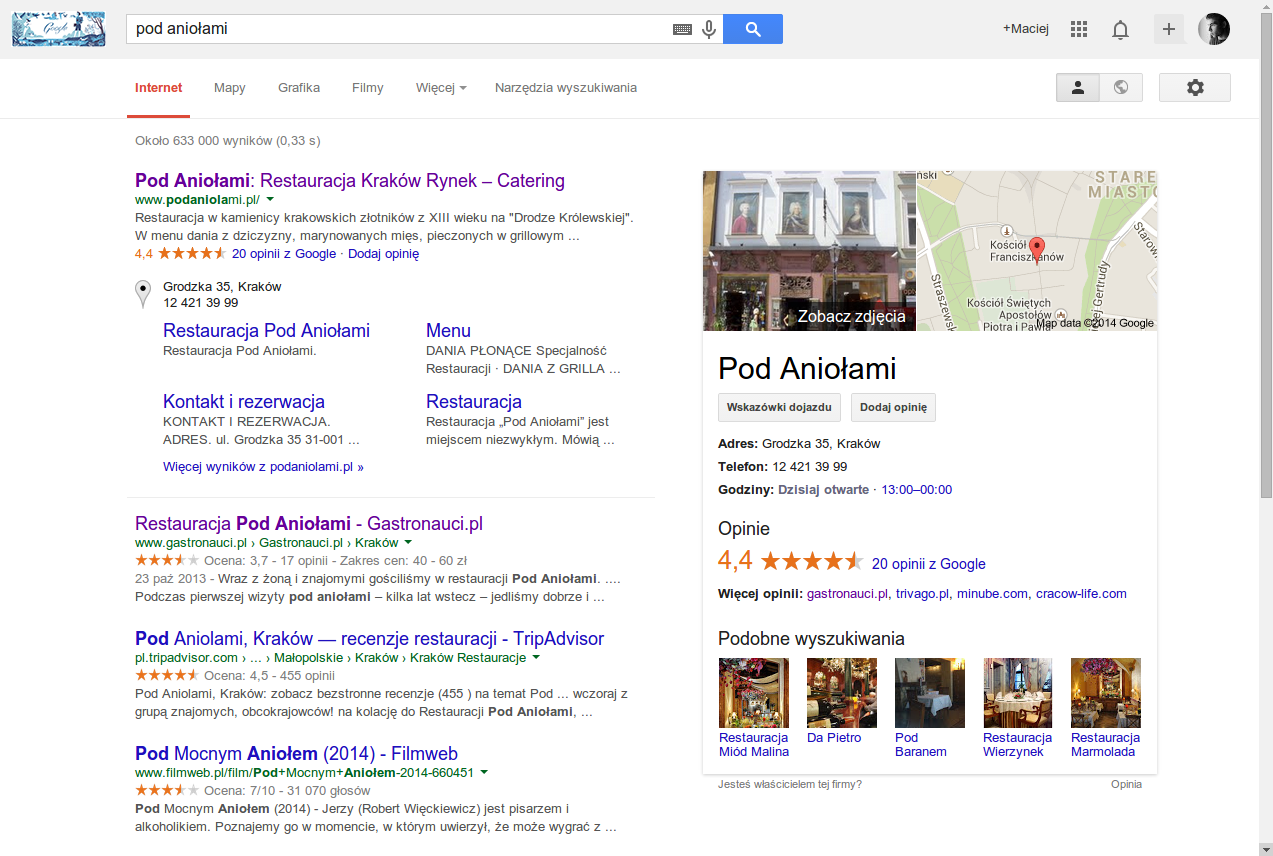
\includegraphics[width=1.0\textwidth]{images/search-result-company-in-google-search-engine.png}
    \captionsource{Wyszukiwanie firmy w~wyszukiwarce Google}{Opracowanie własne.}
    \label{fig:search-result-company-in-google-search-engine}
\end{figure}

%--------------------------------------

\subsection{Rodzaje zależności XY}
\lipsum[6-10] All is according to \parencite{url:zaraz-po-instalacji}.

\begin{figure}[!h]
\centering
\begin{subfigure}{.5\textwidth}
  \centering
  
\includegraphics[width=.4\linewidth]{images/googleplus_color.png}
  \caption{Logo tekstowe}
  \label{fig:google-logo-tekstowe}
\end{subfigure}%
\begin{subfigure}{.5\textwidth}
  \centering
  \scalebox{0.7}
  {
      
\includegraphics[width=.4\linewidth]{images/google-plus-logo.png}
  }  
  \caption{Logo graficzne}
  \label{fig:google-logo-graficzne}
\end{subfigure}
\captionsource{Rodzaje logotypów występujących na witrynie Google+}{\url{https://plus.google.com/}}
\label{fig:logo-google}
\end{figure}

\lipsum[30-33]

\